\documentclass[conference]{IEEEtran}
%
% General
%
\usepackage[english]{babel}

%
% Formatting
%
\usepackage{inconsolata}
\usepackage{hyperref}
\usepackage{lettrine}
\usepackage[factor=1700]{microtype}
\usepackage{balance}
\usepackage{afterpage}

\newcommand{\subscript}[1]{\text{\kern0.1em#1}}

%
% Figures
%
\usepackage{graphicx}

%
% Tables
%
\usepackage{array}
\usepackage{booktabs}
\usepackage{multirow}
\usepackage[flushleft]{threeparttable}

\newcolumntype{L}[1]{>{\raggedright\let\newline\\\arraybackslash\hspace{0pt}}m{#1}}
\newcolumntype{C}[1]{>{\centering\let\newline\\\arraybackslash\hspace{0pt}}m{#1}}
\newcolumntype{R}[1]{>{\raggedleft\let\newline\\\arraybackslash\hspace{0pt}}m{#1}}

\newcolumntype{=}{>{\global\let\currentrowstyle\relax}}
\newcolumntype{-}{>{\currentrowstyle}}

%
% Text shortcuts
%
\renewcommand{\sc}[1]{#1}

\newcommand{\ie}{i.e.}
\newcommand{\eg}{e.g.}

\renewcommand{\tt}[1]{\texttt{#1}}

%
% References
%
\newcommand{\eref}[1]{(\ref{equ:#1})}
\newcommand{\fref}[1]{Fig.~\ref{fig:#1}}
\newcommand{\sref}[1]{Sec.~\ref{sec:#1}}
\newcommand{\tref}[1]{Table~\ref{tab:#1}}

\newcommand{\elab}[1]{\label{equ:#1}}
\newcommand{\flab}[1]{\label{fig:#1}}
\newcommand{\slab}[1]{\label{sec:#1}}
\newcommand{\tlab}[1]{\label{tab:#1}}


\title{
  Massive Generation of High-Quality Power and Temperature Traces of
  Multiprocessor Systems
}

\author{%Ivan Ukhov, Diana Marculescu, Petru Eles, and Zebo Peng
}

\begin{document}
  \maketitle

  \begin{abstract}
    We present a software framework for a rapid generation of realistic power and
temperature traces of multiprocessor systems. The target audience of the
framework is research studies that leverage learning techniques in order to
achieve their goals such as those developing power- and temperature-aware
management strategies. In this context, the availability of sufficient large
amounts of data---which are essential for learning and, hence, exploration of
research ideas---is rather elusive, to say the least. The presented framework
aims to fulfill this need, that is, to provide profuse representative data to
learn from. The overarching goal is to enable new and facilitate existing
studies by making it feasible to explore novel or revived, highly promising, but
data-demanding techniques for data analysis and prediction such as artificial
neural networks with deep architectures.

  \end{abstract}

  \begin{IEEEkeywords}
    Machine learning,
    multiprocessor systems,
    power,
    simulation,
    temperature,
    traffic,
    workload.
  \end{IEEEkeywords}

  \bstctlcite{IEEEexample:BSTcontrol}

  \section{Introduction} \slab{introduction}
  \lettrine[findent=0.4em, nindent=0em]{\textbf{P}}{ower} consumption and heat
dissipation are of paramount importance. The two inseparable phenomena dictate
limitations on the usage of electronic devices and magnify the costs pertaining
to the deployment and maintenance of electronic systems. Power is essentially
energy, and energy translates willingly to hours of battery life and zeros in
electricity bills. Temperature, on the other hand, is one of the major causes of
permanent damage \cite{jedec}, which necessitates the deployment of adequate
cooling equipments, escalating the overall expenses \cite{chaudhry2015}. The
situation is deteriorated even further by the power-temperature interplay:
higher power leads to higher temperature, and higher temperature strikes back by
making devices consume even more power \cite{liu2007}. Under these
circumstances, it is no surprise that power and temperature have steadily been
in the research limelight and have no plans on leaving this spot.

In this paper, we set out to assist researchers working with power and
temperature in one specific but rather broad context. More concretely, we would
like to facilitate the development of on-chip, data-driven, power- and
temperature-aware solutions for multiprocessor systems. Let us clarify the terms
involved in the previous statement; the approach itself will be described
shortly after. \emph{On-chip} refers to taking decisions online or,
equivalently, at runtime, which is in contrast to having decisions taken
offline, at design time. \emph{Data-driven} refers to the usage of machine
learning \cite{bishop2006}, that is, to the usage of algorithms that learn from
data as opposed to algorithms of any other kind. \emph{Power-aware} refers to
decision-making that takes into account the impact on and the impact of power
(and energy) consumption. Similarly, \emph{temperature-aware} refers to
considering heat dissipation when taking decisions.

We approach the outlined objective by developing a methodology for a fast
synthesis of realistic power and temperature profiles. Our motivation for doing
so is described in the next section, \sref{motivation}, and here we only would
like to remark that data-driven techniques obviously require data to learn from,
and these data might not be easily accessible to researchers for a variety of
reasons, preventing research ideas from flowing freely. The goal of this work is
to eliminate this obstacle.

It is important to realize right from the start that, while artificial data
enable thoughts and ideas to evolve and ripen, the solution being developed will
eventually have to face real data. Therefore, the solution should be tested and,
if needed, calibrated in a stage environment prior to the deployment to a
production environment, which could also be done periodically at the end of a
large development cycle. The usage of synthetic data substantially speeds up the
development process due to the flexibility and fast feedback enabled by such
data, which, in particular, means that one can filter out bad ideas at early
stages and focus solely on the ones which are viable.

The remainder of the paper is organized as follows. The motivation for embarking
on this line of research is given in \sref{motivation}.
Section~\ref{sec:prior-work} provides an overview of the prior work. In
\sref{present-work}, the contributions of the present work are summarized. The
addressed problem is formalized in \sref{problem-formulation}. The proposed
methodology and the corresponding toolchain are described in \sref{methodology}
and \sref{toolchain}, respectively. The usage of our technique is discussed in
\sref{guidelines}. Section \ref{sec:conclusion} concludes the paper.


  \section{Prior Work}
  Sniper \cite{carlson2011}.
  \sc{McPAT} \cite{li2009}.
  HotSpot \cite{skadron2004}.
  \sc{3D-ICE} \cite{sridhar2010}.

  \section{Our Contribution}

  \section{Modeling}
  \subsection{System}

  \subsection{Traffic}
  A multifractal wavelet model \cite{riedi1999}.

  \subsection{Workload}
  \sc{PARSEC} \cite{bienia2011}.
  \sc{SPEC CPU2006} \cite{cpu2006}.

  \section{Simulation}
  \subsection{Performance}
  Sniper \cite{carlson2011}.

  \subsection{Power}
  McPAT \cite{li2009}.

  \subsection{Temperature}
  HotSpot \cite{skadron2004}.
  \sc{3D-ICE} \cite{sridhar2010}.
  \cite{ukhov2012}.

  \section{Implementation}
  The toolchain has been implemented in the Rust programming language
\cite{rust}.\footnote{Rust is a systems programming developed by Mozilla
Research and thousands of independent contributors from all around the world.
Rust focuses on memory safety without garbage collection, concurrency without
data races, abstractions without overhead, and stability without stagnation.} It
consists of a number of programs, and the programs are composed of a number of
stand-alone packages. The toolchain also makes use of third-party software.
Regardless of the origin, each component of the toolchain is open source. The
code written by us is distributed under the \sc{MIT} license \cite{mit} and is
available at \cite{sources}. Feedback is welcome, and contribution will be very
much appreciated.

The main programs of our toolchain are called \recorder\ and \streamer, and we
shall describe them next.

\subsection{Recorder}
\begin{figure}
  \centering
  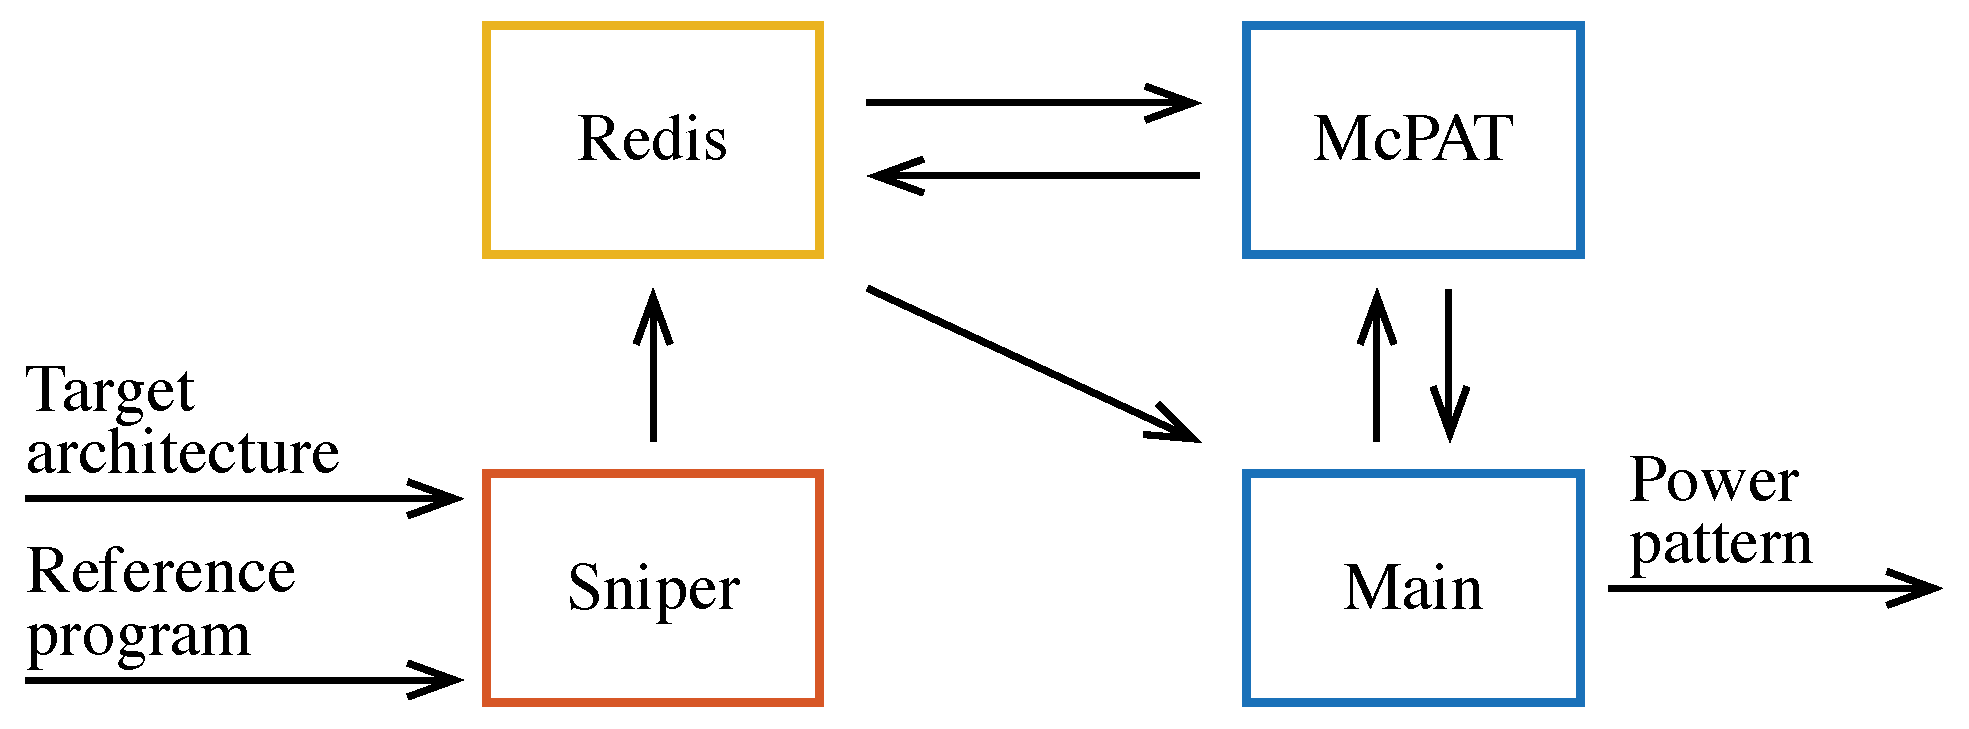
\includegraphics[width=1.0\columnwidth]{include/assets/figures/recorder.pdf}
  \caption{
    The recording infrastructure. The Recorder tool corresponds to the two blue
    boxes on the right-hand side of the figure.
  }
  \flab{recorder}
\end{figure}

\begin{table}
  \begin{threeparttable}
    \caption{Target architecture}
    \begin{tabular*}{\linewidth}{=L{70pt}l}
      \toprule
      Component    & Description \\
      \midrule
      Core         & 2660 MHz, 1.2 V \\
      L1-I/D cache & 32 KB, 4-way, LRU, private \\
      L2 cache     & 256 KB, 4-way, LRU, private \\
      L3 cache     & 8192 KB, 16-way, LRU, one per four cores \\
      \bottomrule
    \end{tabular*}
    \tlab{target}
    \begin{tablenotes}
      \item A detailed description of the target architecture can be found in
      the \texttt{nehalem.cfg} and \texttt{gainestown.cfg} configuration files
      of Sniper.
    \end{tablenotes}
  \end{threeparttable}
\end{table}
% vim: nowrap tw=0

As the name suggests, the purpose of \recorder\ is recording. More specifically,
the tool records reference workload patterns, which are needed as an input to
\streamer. The recording infrastructure is depicted in \fref{recorder}.

The performance simulator is Sniper \cite{carlson2011}.

The power simulator is \sc{McPAT} \cite{li2009}.

The key-value storage is Redis \cite{redis}.

The database is SQLite \cite{sqlite}.


\subsection{Streamer}
\begin{figure}
  \centering
  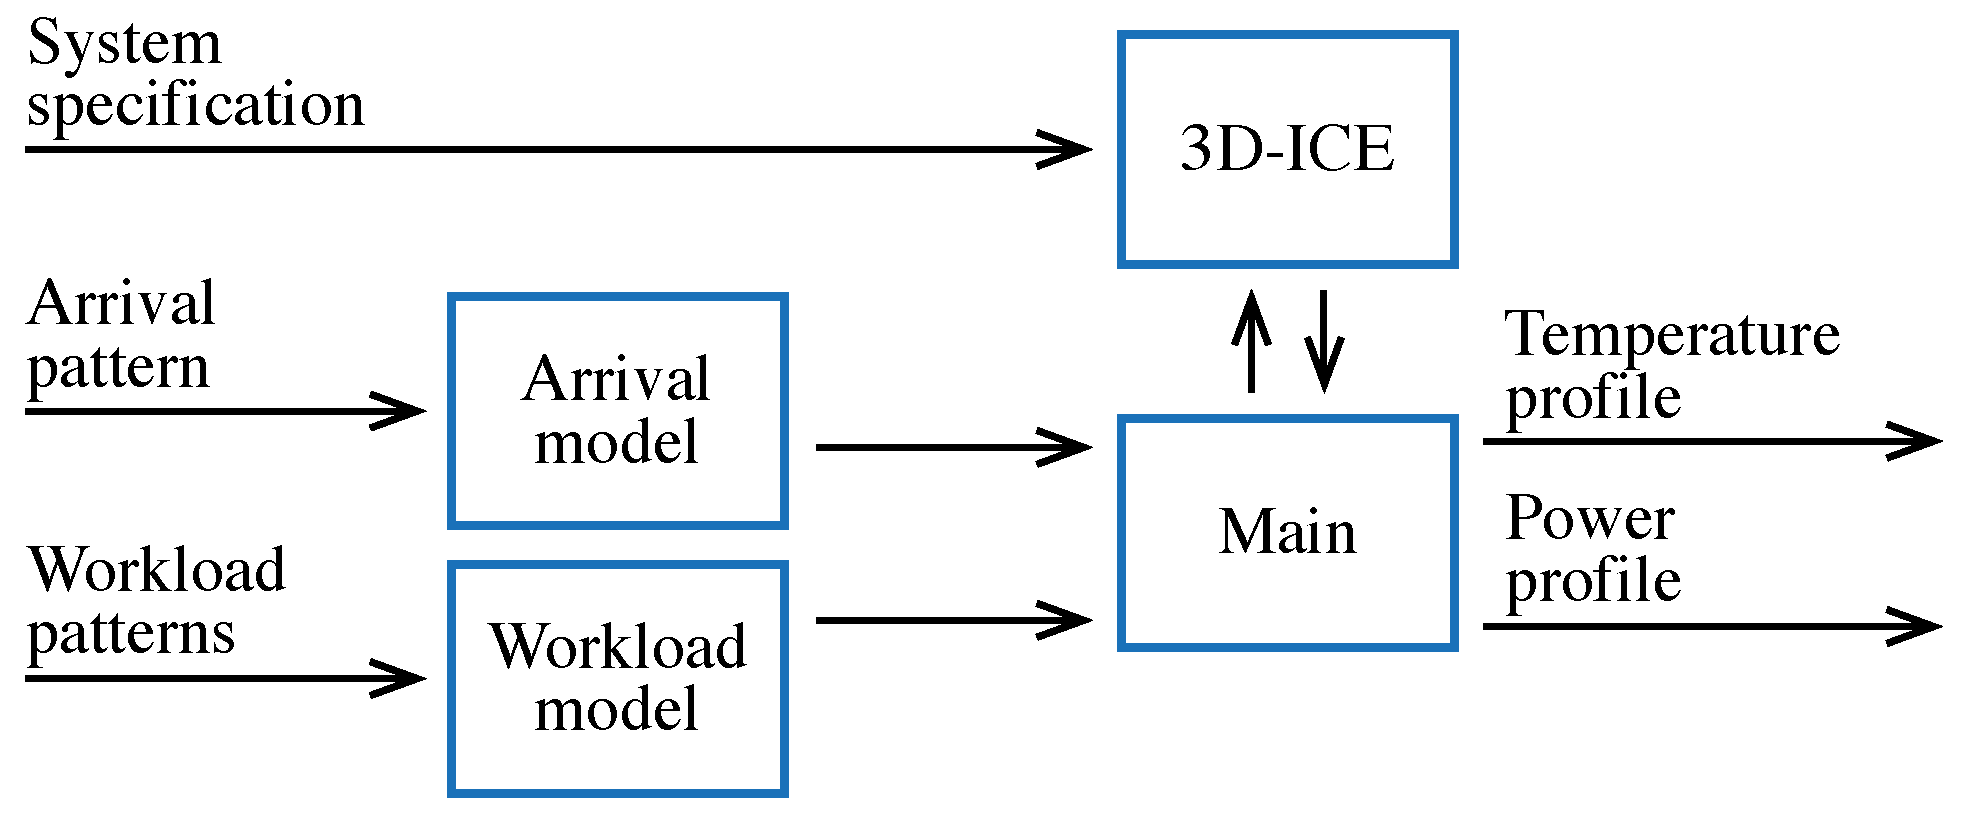
\includegraphics[width=1.0\columnwidth]{include/assets/figures/streamer.pdf}

  \caption{The Streamer tool. \emph{System specification} refers primarily to
  the information about the thermal package and floorplans of the platform,
  which are needed for temperature simulation. \emph{Job model} refers jointly
  to the traffic and workload models (\sref{traffic} and \sref{workload}).}

  \flab{streamer}
\end{figure}

The Streamer tool corresponds to the data-synthesis stage, which means that it
is responsible for synthesizing power and temperature data using reference data
as a material for the synthesis; see the module labeled ``Streamer'' in
\fref{methodology}. The structure of the tool is laid out in \fref{streamer}.

Given a traffic pattern and a set of workload patterns, Streamer proceeds as
follows. The traffic pattern is processed as it was described in \sref{traffic},
which results in an adequately configured multifractal wavelet model
\cite{riedi1999}. The model is then used to generate a stream of arrival times.
The arrival times are fleshed out using the workload patterns, which was
explained in \sref{workload}. The result is a stream of jobs, and the whole
operation is referred to as job modeling in \fref{streamer}. The rest follows
\sref{composition}. The job stream is handled by a scheduling policy; in
\fref{streamer}, this policy is a part of the Main module. As the incoming jobs
are being scheduled, the power profile of the system under consideration is
being constructed. The power profile is piped into a temperature simulator (to
be discussed below), which delivers a temperature profile. The continuity of the
process is worth noting: just as with arrival times and jobs, power and
temperature can be viewed as streams of data. The synthesized data (power and
temperature) can be fed back to the scheduler and/or stored for later usage. In
the latter case, similar to reference data, the output is an SQLite database.

Let us now outline how temperature simulation is undertaken inside Streamer. The
simulation is based on the popular thermal \sc{RC} model. In this paradigm, a
so-called thermal \sc{RC} circuit representing the system at hand is constructed
and then used to analyze the thermal behavior of the system. The analysis boils
down to solving a system of differential equations, which can be done using
different integration techniques. In our case, the solution is based on a solver
leveraging exponential integrators \cite{hochbruck2010, ukhov2014}. The
construction of thermal circuits is outsourced to either HotSpot
\cite{skadron2004} or \sc{3D-ICE} \cite{sridhar2010} (see \fref{streamer}). Both
simulators are based on the thermal \sc{RC} model, and we extract the circuits
that they build, which results in a unified interface for working with the two
alternatives.

To summarize this subsection, the Streamer tool produces streams of power and
temperature data, and this procedure closely follows the ideas presented in
\sref{methodology}. Our temperature simulation is based on the thermal \sc{RC}
model, in which thermal circuits are constructed by either HotSpot or
\sc{3D-ICE}.



  \section{Experimental Results}

  \section{Conclusion}
  In this paper, we emphasized the need for developing tools for studying
electronic systems with data-driven applications in mind. We argued that the
techniques capitalizing on learning from data have special requirements, and
that the state-of-the-art simulators are unable to fulfill them due to
prohibitively large simulation times. Acknowledging the importance of power and
temperature for the design of multiprocessor systems, we developed a methodology
for fast generation of synthetic power and temperature traces that preserve the
idiosyncrasies of their real-life counterparts. Last but not least, we
implemented a toolchain that embodies the presented approach, which was
subsequently assessed and shown to be extremely fast.


  \section*{Acknowledgments}
  The authors would like to acknowledge everybody.


  \begingroup
    \bibliographystyle{IEEEtran}
    \bibliography{IEEEabrv,include/references}
  \endgroup
\end{document}
